\section{Design}

\subsection{Klasserelationer}
Den avancerede versions design er også baseret på Model-View-Controller-conceptet, og indeholder derfor pakkerne, \textit{model}, \textit{view} og \textit{control}. Klasserne i control-pakken er uafhængige af klasserne i de andre pakker, men oprettes og tildeles i view-klasser, der giver kontrol over spillets progression og brugergrænsefladens udseende.

I \textit{Driver}-klassen, hvori main-metoden for programmet ligger, oprettes kun et \textit{ViewFrame}-objekt, der nedarver fra JFrame, og viser spillets vindue. I denne klasses constructor oprettes alle andre relevante klasser, som findes i view-pakken [REFERENCE TIL KLASSEDIAGRAM]. Disse nedarver fra JPanel, og tilføjes og fjernes fra JFramen afhængig af hvor i programmet spilleren befinder sig. Er spilleren f.eks. i hovedmenuen, bruges \textit{MenuPanel}-panelet, mens \textit{HeaderMultiplayerPanel} og \textit{BoardMultiplayerPanel} tilføjes, hvis spilleren er i multiplayer-delen af spillet. På denne måde har hver scene i spillet en eller to tilhørende klasser der nedarver fra JPanel. 

Spilleren navigerer vha. JButtons eller tastatur-input der modtages i control-klasserne. Control-klassen \textit{ViewFrameListener} oprettes ligeledes i \textit{ViewFrame}s constructor, hvorefter den som KeyListener tilføjes til alle panelerne. Denne klasses funktioner er globale, da den står får `mute'- og `return to menu'-funktionerne, der konstant skal være tilgængelige for spilleren, uafhængig af de viste paneler.


Hvert panel opretter også i deres egne constructors deres tilhørende Listener fra control-pakken. Disse Listeners står for kontrollen, der er unik for deres panel. Alle panel-klasserne oprettes med \textit{ViewFrame} som parameter, der derefter igen bruges som parameter, når panel-klassens control-klasse oprettes. Control-klassen kan derefter bruge \textit{ViewFrame}, til at skifte paneler ud, når knapper eller taster trykkes. Specielt for \textit{MenuListener}, der hører til hovedmenu-panelet, oprettes i constructoren også et \textit{GameSingleplayer}- og et \textit{GameMultiplayer}-objekt, da disse skal bruges, når der klikkes på `Singleplayer'- eller `Multiplayer'-knapperne. 

\textit{GameSingleplayer} og \textit{GameMultiplayer} er underklasser til \textit{Game}-klassen, og står for spil-delens oprettelse ved at bruge de andre objekt-klasser i model-pakken: \textit{Board}, \textit{Food} og \textit{Snake}. Derudover findes der i model-pakken hjælpeklasserne: \textit{Field}, \textit{Direction}, \textit{Event} og \textit{Player}. \textit{Game} extends Observable-klassen, der gør det muligt for view-klasserne at blive notificeret, når der foretages ændringer i spillet, og følgelig tilpasse sig ændringerne i brugergrænsefladen.

Al grafik, som ikke er fra \textit{Swing}-biblioteket, er importeret i klassen \textit{Images}, giver enhver view-klasse adgang til at få fat i alle billeder. På samme måde er selv-definerede farver oprettet i klassen \textit{Colors}.


\subsection{Multiplayer}
Multiplayer ligner singleplayer rigtig meget. De forgår begge med slanger på samme board.  Problemet med at integrere multiplayer ind i vores singleplayer kodebase er at de steder hvor at multiplayer ikke ligner singleplayer er meget spredt.

Man kunne sige at singleplayer og multiplayer kunne dele 90\% af koden, men de resterende 10\% er flettet ind i de 90\%. For eksemple har multiplayer et lidt anderledes score system, så single og multiplayer headeren som viser score kræver lidt anderledes tekst. Det samme gælder for slange farve valg, hvor at der nu er to slanger. Multiplayer delen skal nok også have lidt anderledes gameplay. Det kan også betyde at den måske har noget ekstra slange mad eller en lidt anderledes slange. 

Vores mål for multiplayer designet var forståelighed og at genbruge mest muligt kode mellem single og multiplayer. Vi overvejede at bruge en kombineret single og multiplayer klasse som kunne holde et array af slanger. Så hvis der var to slange ville vi bruge multiplayer gameplay og singleplayer gameplay når der var en. Fordelen ved dette ville være at view delen i MVC, bare kunne loope over nogle array lige meget om det var single eller multiplayer. Vi ville også nemt kunne tjekke om vi var single eller multiplayer. Det ville bare være en if statement om der er en eller to slanger. Det vil også være nemt at tilføje for eksemple 10 slanger/spillere. Ulemperne ved dette er at forskellen på single og multiplayer er meget lille. Vi kan genbruge en hel masse kode mellem dem, men er det det bedste hvis det resultere i en masse if singleplayer then ... else statements? Et mere forståeligt design ville have en adskillelse af single og multiplayer.

Dette ledte til designet i \figref{game-design} . Vi har lavet to seperate single og multiplayer game klasser som arver fra en abstract game klasse. Fordelen ved dette er at vi har en seperation mellem multi og singleplayer. Det som forgår i singleplayer klasse har ingen indflydelse på multiplayer klassen. Med dette design løber vi ind i problemer når vi skal implementere view og controls i MVC. Det vi har valgt at gøre er at lave en base udgave af hvert komponent. Basen har alt det som er fælles for single og multiplayer. Vi laver så to nye klasser BaseSingleplayer og BaseMultiplayer som nedarver fra base klassen.  De to klasse kan så frit override/udvide implementationerne i base klasserne. 

FIG VISIO!!!!!


\begin{figure}[h]
	\centering
	\graphicspath{ {pics/} }
   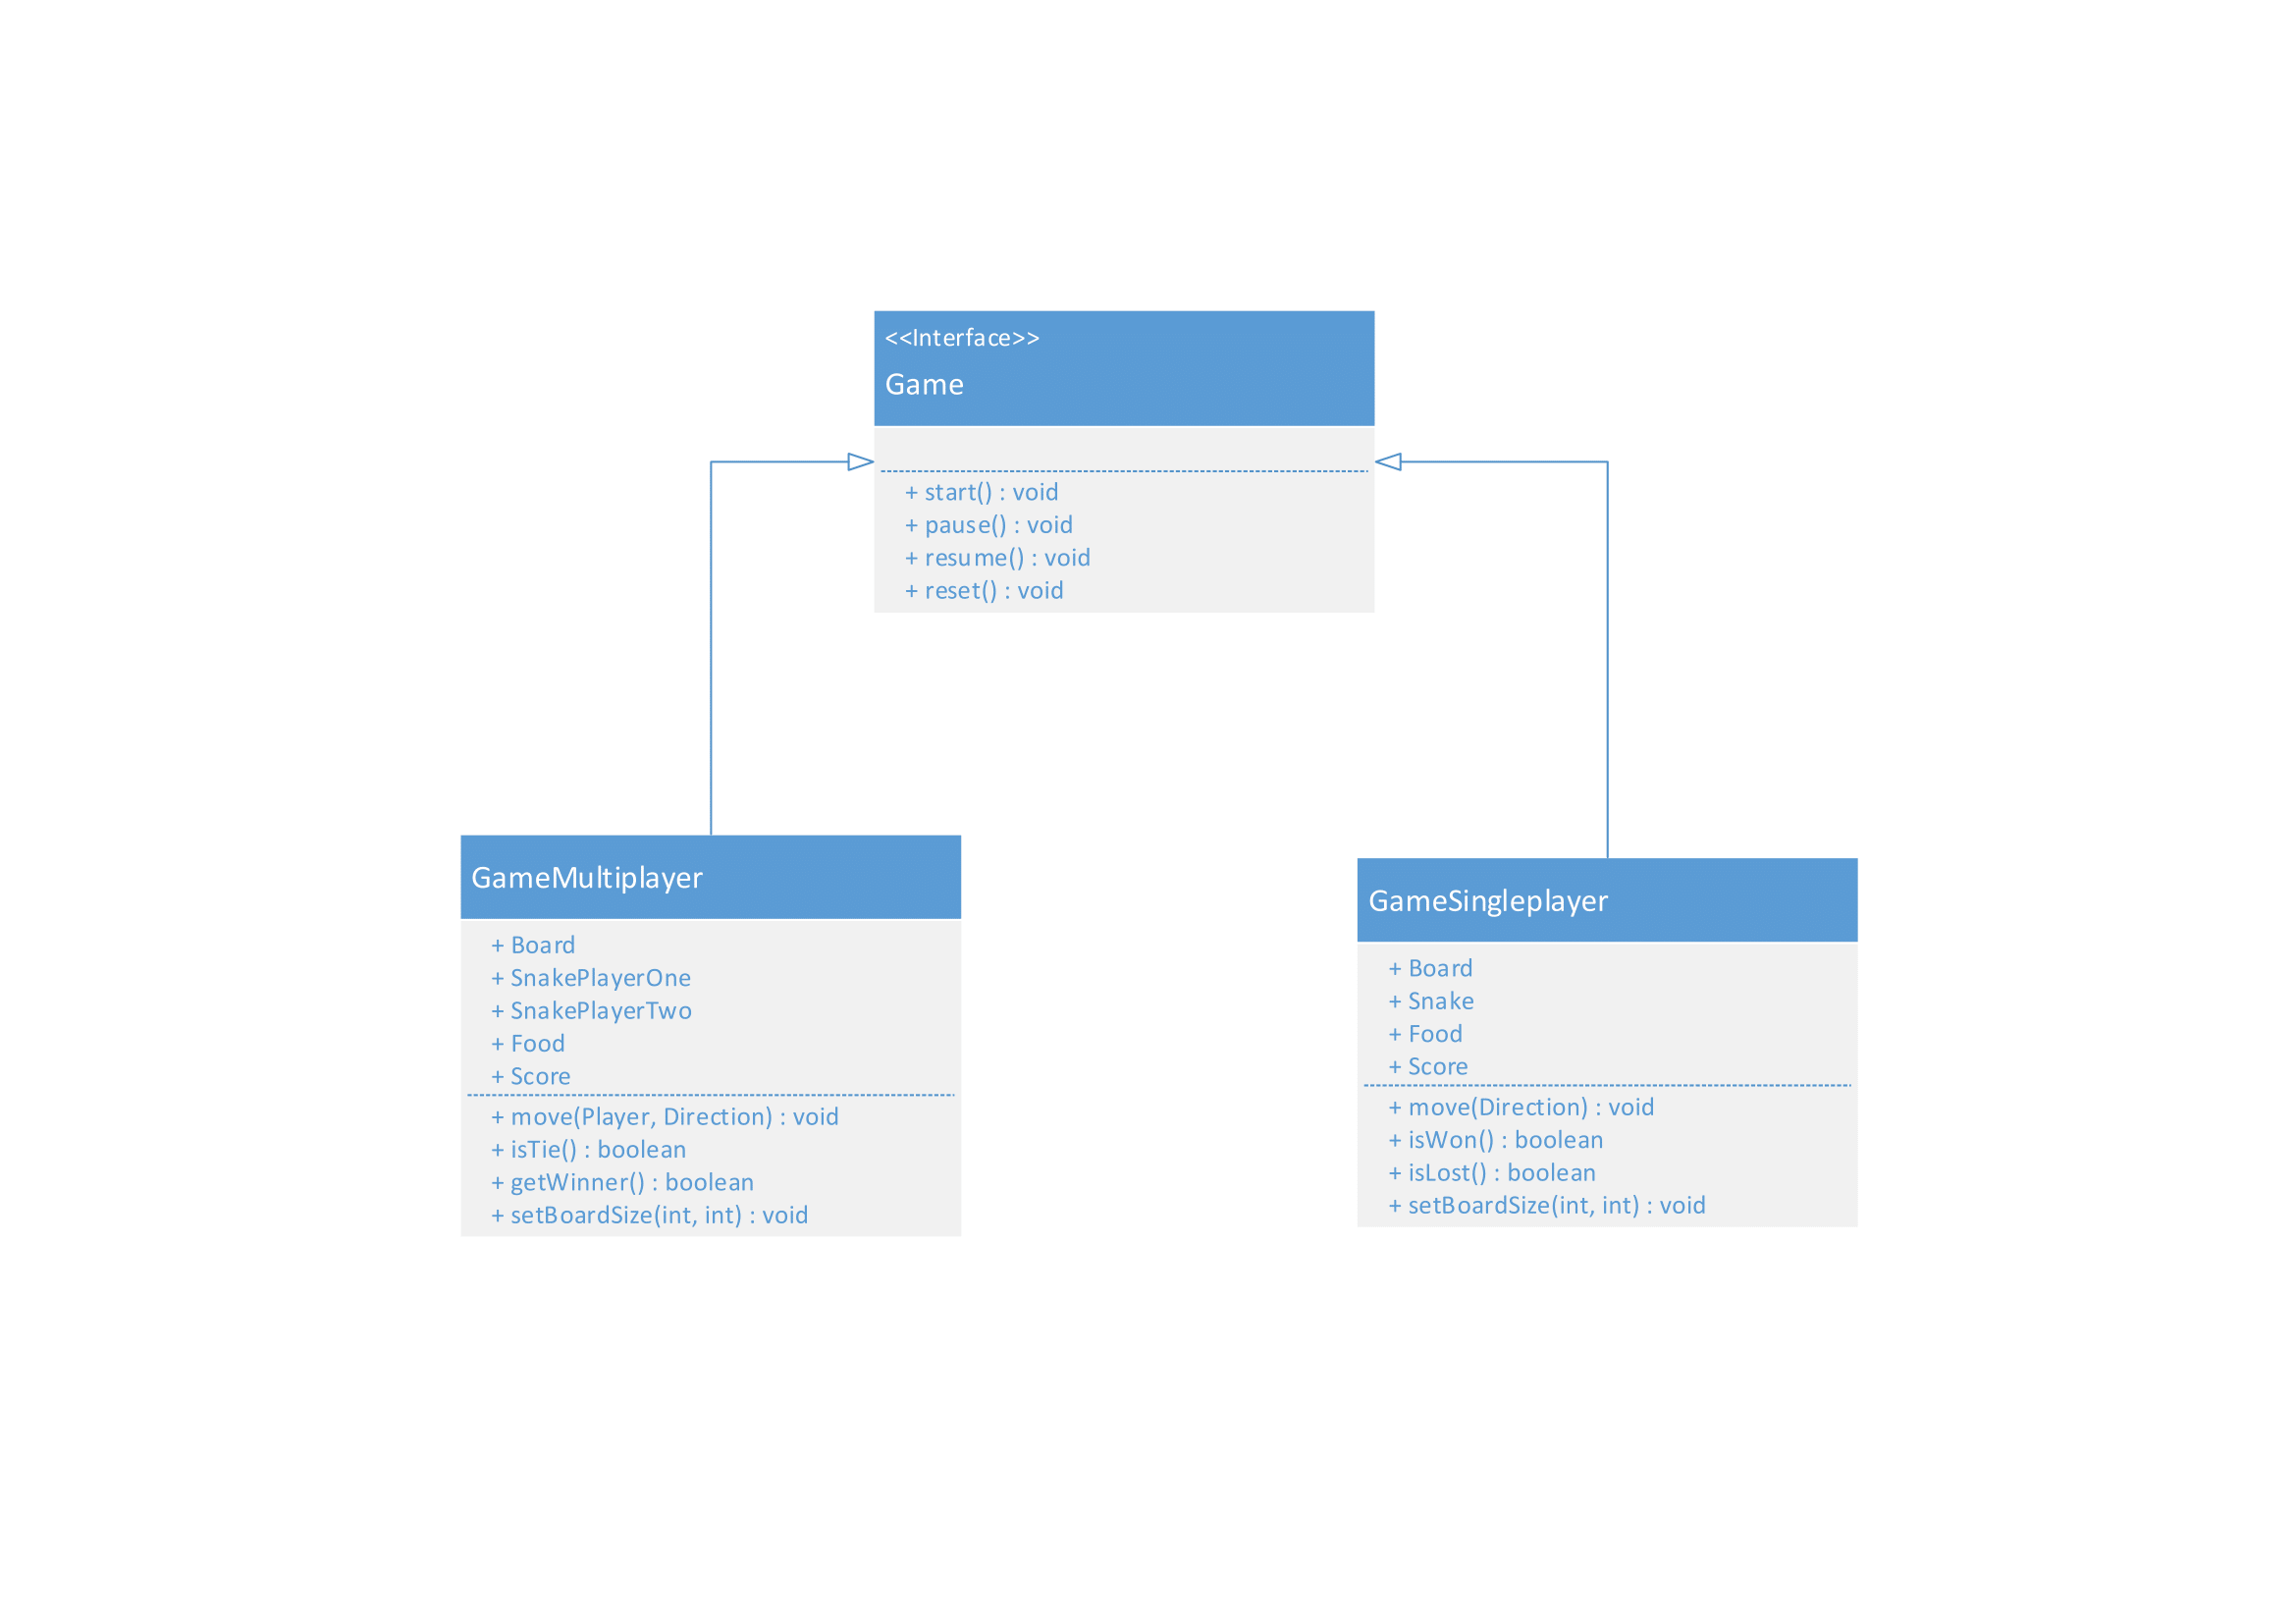
\includegraphics[width=1.0\textwidth]{advanceret/game-design.png}
	\hspace{0.1\textwidth}
	\figlab{game-design}
	\caption{Overview of our multiplayer design.}
\end{figure}

